\documentclass[12pt]{article}
\usepackage[english]{babel}
\usepackage{float}
\usepackage{enumerate, setspace, stackengine}
\usepackage[hidelinks]{hyperref}
%\usepackage[margin=1.5cm]{geometry}
\usepackage{geometry}
\geometry{top=1.5cm, left=1.5cm, right=1.5cm, bottom=1.5cm}
\usepackage{caption, subcaption}
\usepackage{amsmath, amsfonts, amssymb}
\usepackage{fontspec}   %加這個就可以設定字體
\usepackage{xeCJK}       %讓中英文字體分開設置
\usepackage{listings, color}
\usepackage{wrapfig}
\setCJKmonofont{FandolFang-Regular.otf}
\setCJKmainfont{標楷體} %設定中文為系統上的字型,而英文不去更動,使用原TeX字型



\definecolor{dkgreen}{rgb}{0,0.6,0}
\definecolor{gray}{rgb}{0.5,0.5,0.5}
\definecolor{mauve}{rgb}{0.58,0,0.82}

\lstset{frame=tb,
  language=Java,
  aboveskip=3mm,
  belowskip=3mm,
  showstringspaces=false,
  columns=flexible,
  basicstyle={\small\ttfamily},
  numbers=none,
  numberstyle=\tiny\color{gray},
  keywordstyle=\color{blue},
  commentstyle=\color{dkgreen},
  stringstyle=\color{mauve},
  breaklines=true,
  breakatwhitespace=true,
  tabsize=3
}



\title{\textbf{Real Time System}\\ Project\#1}
\author{Team7 - R04922058 鄭以琳 , R04922034 吳軒衡}
\date{}

\begin{document}
\maketitle

\section{Part I: Linux Kernel Building}
\subsection*{Kernel Building Steps}
	In this section, the fundamental steps required to build a kernel are examined.
\begin{enumerate}
\item \verb|Install the Requried Pacakges && Get the Source Code|\\
'sudo apt-get install fakeroot build-essential kernel-package libncurses5 libncurses5-dev'
\begin{itemize}
\item fakeroot:\\
	fakeroot is a package that allows a normal user to fake itself as root in order to prevent the need of changing permissions of files when building an archive. fakeroot start up a shell and fake all the permission related such as chown , chgrp operation by simulation, and nothing happens to the actual permission of the files. When building a kernel package, we require some of the scripts and codes to be owned root, but we don't want to be limited to archive the package with root permission, and fakeroot comes into use.
\item build-essential:\\
	build-essential is a set of tools that is required to build a debian package, which are defined in the debian policy manual. It is related to a set of compilers as well as GNU Libraries. A few examples are : dpkg-dev ,g++ , gcc ,libc and make.
\item kernel-package:\\
	This package is capable of handling the steps required to compile a kernel using make-kpkg, and it also helps to maintain multiple version of kernels in a single machine without fear of contaminating one another. It also allows user to create kernel-headers.
\item libncurses5 and libncurses5-dev:\\
	libncurses libraries are used to render graphical user interface on terminal, such as the one we see when executing 'make menuconfig'.
\end{itemize}	
\item \verb|Clean up the Source Code|\\
	'make mrproper'\\
	Clean up all the settings as well as the temporary files such that we get a clean source code. 'make mrproper' will remove the .config generated by 'make menuconfig' as well as the tmporary .o files.
	This is different from 'make clean', which removes the .o files only.

\item \verb|make menuconfig|\\
	make menuconfig will read the Kconfig files,presents a libncureses generated user interface for user to configure the kernel and save the final configuration in .config file.\\
	Possible configurations for each module are 
\begin{itemize}
	\item \verb|[*] include|\\
		Included modules will be compiled into the kernel.
	\item \verb|[ ] exclude|\\
		Excluded modules will not be compiled into the kernel , nor will them be compiled separately into loadable modules.
	\item \verb|[M] modularized|\\ 
		Modularized modules will be compiled in the 'make module' step and installed in the 'make module install' step.
\end{itemize}
\item \verb|Compile the Kernel|\\
	'make bzImage'\\
	make bzImage will create a bzImage file under /arch/\$ARCH/ where bzImage stands for big zImage that is compressed by gzip, not bzip. This is loaded by the boot-loader onboot.

\item \verb|Compile the Modules|\\
	'make modules'
	This step compiles all modules that are configured as modularized in the 'make menuconfig' step. 

\item  \verb|Install the Modules to Kernel|\\
	'make module\_install'
	This step copies all the compiled modules into the lib/modules/\$kernel\_version/ directory.

\item \verb|Setup the Kernel for Boot|\\
	'make install'\\
	make install will create System.map, initrd.img and config under the directory /boot. The bzImage file generated at 'make bzImage' step will be copied to /boot/ and renamed as vmlinuz. The older version of the kernel will be renamed as vmlinuz.old
	\begin{itemize}	
	\item vmlinuz is a compressed version of vmlinux by zlib, which is decompressed at boot up. \footnote[1]{zlib is a software library use for data compression, an abstraction of the DEFLATE compression algorithm used in gzip file compression program, there fore a simple renaming of bzImage works.}

	\item initrd.img  is a minimum Linux ram-disk image that is mounted by the bootloader to mount all other modules and execute /sbin/init.

	\item System.map is a symbol table used by the kernel, required by processes such as klogd , lsof , ps and so on.
	config is a copy of the .config file.
	\end{itemize}


\item \verb|Update Grub for future Booting|\\
	uncomment grub\_hidden\_timeout and update-grub2\\
	Uncommenting the grub\_hidden\_timeout related settings allow users to switch between various versions of Linux to boot into.
\end{enumerate}
\newpage
\section{Part II: Linux Scheduling Policy Testing}
\subsection*{Linux Scheduling Concepts}
	Linux determines which thread to run next based on each thread's \verb|sched_priority| value. Threads scheduled using real-time policies (\verb|SCHED_FIFO|, \verb|SCHED_RR|) can have a priority value from 1(low) to 99(high). Priority values of normal scheduling policies (\verb|SCHED_OTHER|, \verb|SCHED_BATCH|, \verb|SCHED_IDLE|) are always 0(lowest). Since the scheduling in Linux is preemptive, real-time jobs can always preempt non-real-time jobs.
	
	By default, threads are scheduled by \verb|SCHED_OTHER| policy, however, Linux provides some system calls for users to change the policy for a certain thread. In this project, we are asked to create threads scheduled by FIFO. Since a \verb|SCHED_FIFO| thread can run as long as it wishes without time slicing, which may block other threads forever, it requires root privileges to activate this policy.
	
\subsection*{Implementation}
	We used Pthreads library to implement the multi-thread C program.
\paragraph{Change the scheduling policy}\mbox{}\\
First, we called \verb|setFIFO()| function to change main thread's scheduling policy to FIFO. The code snippet is shown below:
	
\begin{lstlisting}[language=C++]
void setFIFO(){
	struct sched_param param;
	param.sched_priority = sched_get_priority_min(SCHED_FIFO);
	sched_setscheduler(0, SCHED_FIFO, &param);
}
\end{lstlisting}
There are two system calls in this function:
\begin{enumerate}
	\item \verb|sched_get_priority_min(int policy)|\\
		This function returns the minimum priority value that can be set using \verb|policy|. It usually returns 1 when \verb|policy = SCHED_FIFO|.
	\item \verb|sched_setscheduler(pit_t pid, int policy, const struct sched_param *param)|\\
		This function sets scheduling policy and the associated parameters for the thread specified by \verb|pid|. \verb|pid=0| refers to current thread.
\end{enumerate}
\paragraph{Inherit scheduling attribute}\mbox{}\\
Second, instead of individually setting the scheduling policy for each new thread, we used \verb|PTHREAD_INHERIT_SCHED| to specify that each thread should inherit its scheduling policy from the parent.
\begin{lstlisting}[language=C++]
pthread_attr_t attr;	
pthread_attr_init(&attr);	
pthread_attr_setinheritsched(&attr, PTHREAD_INHERIT_SCHED)
pthread_create(&thread, &attr, ...);	

\end{lstlisting}

\newpage
\subsection*{Discussion}
\paragraph{FIFO scheduling}\mbox{}\\
With the FIFO scheduling policy, a thread can run as long as it wishes unless one of these conditions occurs:
\begin{enumerate}
	\item It is blocked (ex: I/O, mutex).
	\item It is preempted by a higher priority thread.
	\item It volunteers to give up control of processor (ex: sleep, yield).
\end{enumerate}
Therefore, we can't implement "busy for one second" by sleep() function in this project. Calling sleep will remove the current thread from runqueue even if it is scheduled by FIFO. Our solution is to use clock() function with a while loop, which continuously checks the number of clock cycles already used until a second has elapsed.  
\paragraph{CPU affinity}\mbox{}\\
Setting CPU affinity forced a thread to run on assigned CPU(s). Each CPU has its own runqueue. Without setting affinity, threads can be put in different FIFO queue and execute simultaneously, which is not the result we want in this project. A way to solve this problem is using \verb|pthread_setaffinity_np()| function. According to Linux manual, child process will inherit parent's CPU affinity by default, so we only need to specify main thread's affinity. 
 
\subsection*{Result}
\begin{figure}[h]
	\centering
	\begin{minipage}[b]{0.4\textwidth}
		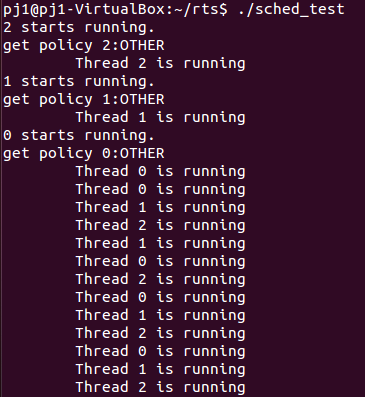
\includegraphics[width=\textwidth]{fig_default}
		\caption[Caption for the list of figures]{Default}
		\label{fig:default}
	\end{minipage}
	~
	\begin{minipage}[b]{0.52\textwidth}
		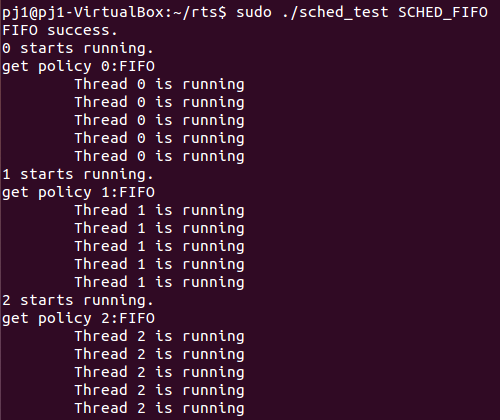
\includegraphics[width=\textwidth]{fig_fifo}
		\caption[Caption for the list of figures]{FIFO}
		\label{fig:fifo}
	\end{minipage}
\end{figure}

\end{document}
